% ===========================================================================
\section{Discussion}
\label{sec:discussion}

\subsection{Format Dependence as Measurement Challenge}
\label{sec:format-crisis}

On identical items, MC understates BBQ safety by 16~pp, understates sycophancy resistance by 19~pp, overstates MMLU capability by 9~pp, and leaves AI factual recall at $-1$~pp (Section~\ref{sec:format-dependence}).  Sign reverses across properties, which buries any single-factor explanation: judge leniency, length, evasion, and item difficulty all predict a monotonic direction, and the data are not monotone.  MC and OE elicit related but distinct behaviours, and current safety practice~\cite{parrish2022bbq} publishes only one of the two --- the one whose particular channel the optimisation gradient happens to be calibrating against.

\subsection{Scaffold Effects: What Survives and Why}
\label{sec:scaffold-discussion}

Scaffold architecture sorts the safety contrast on the four-benchmark mix tested; aggregating across configurations produces no uniform effect.  ReAct and multi-agent each pool inside the pre-registered $\pm 2$~pp TOST equivalence margin (RD$\,=\,-0.7$ and $-0.6$~pp respectively), and map-reduce pools well outside it ($-7.3$~pp, NNH~14) (Table~\ref{tab:confirmatory}).  Architecture matters.  The classical-significance category that multi-agent occupies flips across scoring methods while its TOST classification holds throughout, which is why effect-size interpretation should take precedence over dichotomous significance testing for deployment decisions.

The map-reduce technique eliminates MC options from sub-calls.  MC vs.\ OE itself produces variation in measured safety that ranges from 5 to 20~pp on the same items (Section~\ref{sec:format-dependence}).  The scaffold result is a reformulation of the format result.  By propagating MC options most of the loss can be recovered; the remaining loss is due to semantic invocation rather than chain structure (Section~\ref{sec:reframing-scaffold}).

GPT-5.2 has the smallest format difference of any model on the sycophancy test ($+2.9$~pp) and the second-largest collapse on bias-invoked semantics ($-13.0$~pp under aggressive invocation in Phase~2).  Dose-response replicates across six models.  Surviving the format tests or the semantic tests does not guarantee survival of both.

\paragraph{Sycophancy fits the depth-of-encoding pattern.}
Sycophancy supplies the strongest empirical fit (Section~\ref{sec:sycophancy-scaffold}).  The lowest-baseline property is also the only one where all three scaffolds improve resistance, and the bidirectional model$\times$configuration interaction (Table~\ref{tab:sycophancy-rates}) recasts ``scaffolds harm safety'' as ``scaffolds redistribute safety,'' compressing the gap between high-baseline and low-baseline properties.

\paragraph{Alternative explanations for the depth-of-encoding pattern.}
The baseline--robustness correlation is a descriptive regularity; ``depth of encoding'' names the pattern without explaining it.  Four non-Goodhart explanations deserve consideration.

\emph{Benchmark difficulty.}  If sycophancy items are generally harder, lower baselines and greater perturbation sensitivity would co-occur regardless of encoding quality.  Two controls argue against this being the dominant mechanism.  First, AI factual recall at an intermediate baseline (77.0\%) shows zero sensitivity to all three perturbation types.  Second, MMLU and BBQ at nearly identical baselines (${\sim}85$\%) show format effects in opposite directions ($-9.2$~pp vs.\ $+16.2$~pp); properties at comparable difficulty produce qualitatively different perturbation profiles, so difficulty alone cannot explain the baseline--robustness correlation.

\emph{Variance compression.}  A second potential concern is whether the observed relationship between baseline robustness and perturbation robustness is due to a statistical variance-compression artefact.  At proportions close to either end of the $[0, 1]$ range, binomial variance contracts, mechanically attenuating effect magnitudes.  Both controls eliminate this possibility.  If variance compression were operative, AI factual recall at 77.0\% baseline should still show some sensitivity proportional to the variance available to be compressed; it shows none.  Similarly, although MMLU and BBQ both sit near an 85\% baseline, they show effect magnitudes in opposite directions ($-9.2$~pp vs.\ $+16.2$~pp), not the similarly sized same-direction effects that variance compression would predict.  A purely variance-compression based model also predicts a monotonically decreasing function of effect magnitude versus baseline rate; our results instead show that properties at the same baseline can be insensitive, diminished or enhanced depending on what construct is measured, which is indicative of property-specific behaviour rather than artefactual scale effects.

We measure baseline rates before applying scaffolding; baseline is therefore an independent predictor, not a circular restatement of the outcome.

\emph{Training data distribution.}  Properties with more alignment training examples would achieve both higher baselines and greater robustness; we cannot test this directly, but the gradient's consistency across six models from four providers with substantially different training pipelines suggests it tracks construct-level properties rather than provider-specific training choices.

\emph{Construct complexity.}  Sycophancy resistance may require balancing competing objectives (helpfulness vs.\ epistemic integrity) in ways that bias avoidance does not.  This overlaps substantially with the depth-of-encoding framing itself: complex constructs may require deeper encoding, which makes the two accounts hard to distinguish empirically.

These four explanations are not mutually exclusive; each likely contributes to portions of the observed gradient.

Property-specific language in scaffold prompts selectively degrades the invoked property.  Opus's near-immunity to bias-invocation in Phase~2 is consistent with deeper encoding for this property in the highest-baseline model ($-2.3$~pp, within the pre-registered $\pm 2$~pp TOST margin).  The framework generates a testable prediction: reasoning-specialised models should show compressed vulnerability ranges.  Surface cues are not the same as grounded reasoning.

\subsection{The Evaluation-Optimisation Gap}
\label{sec:goodhart}

Format dependence (Section~\ref{sec:format-crisis}) and scaffold effects (Section~\ref{sec:scaffold-discussion}) share a common root: evaluation-context specificity.  When safety evaluations conducted via direct API in a fixed response format become the target of alignment optimisation, the resulting safety behaviours calibrate to the evaluation context rather than to the underlying construct~\cite{strathern1997improving}.  Format dependence is the direct consequence; scaffold degradation is the partially overlapping one, driven primarily by format conversion (40 to 89\% of the effect), with a residual reflecting genuine reasoning disruption under task decomposition.

Safety behaviours optimised for MC evaluation contexts produce format-specific response patterns that succeed in evaluation but fail in open-ended deployment (Section~\ref{sec:format-dependence}); and when agentic scaffolds change the effective evaluation context, properties tied to particular evaluation contexts become selectively exposed, producing the depth-of-encoding gradient (Section~\ref{sec:depth-encoding-def}) and the property-specific invocation mechanism (Section~\ref{sec:semantic-invocation}).

Evaluation breadth grows; evaluation depth does not.  NIST AI~800-2~\cite{nistai8002026} and the EU AI Act~\cite{euaiact2024} require neither format-paired safety evaluation nor scaffold-augmented evaluation of the bias/sycophancy/truthfulness benchmarks behind model cards.  The frontier labs took the latter methodology to dangerous-capability assessment a few years ago (Anthropic's RSP first, then OpenAI and DeepMind); the proxy safety benchmarks never made the same move.  Map-reduce degradation (Section~\ref{sec:primary-analysis}) is the resulting context mismatch surfaced --- safety training calibrated for direct-API benchmarks, running inside structure-destroying delegation chains.

Monotherapy reliably selects for resistance~\cite{cdc2019antibiotic}; single-distribution safety training is monotherapy by the same logic (direct API, MC format, single-turn).  Combination therapy removes the failure mode --- format-paired, scaffold-augmented evaluation is the AI-safety analogue.

\subsection{Limitations}
\label{sec:limitations}

\paragraph{Benchmark format scope.}
Three of the four primary safety benchmarks use MC format.  The format dependence finding (Contribution~2) turns this limitation into a strength --- the MC/OE comparison requires MC benchmarks --- but the scaffold analysis inherits the converse confound, with map-reduce degradation partly format-driven.  Construct-validity evidence (option-preserving recovery, AI factual recall control dissociation, and open-ended probes) is reported in Sections~\ref{sec:option_preserving}--\ref{sec:invocation-framework} below.

Scaffold-architecture coverage in this study is non-exhaustive.  Our four configurations (direct API, ReAct, multi-agent critic, and map-reduce) are reasonable defaults, not production-optimised implementations; the tested ReAct in particular omits the calculator, text-search, and scratchpad tools that production ReAct deployments routinely include (deviation D-004 from pre-registration), and the production-faithful version is left to replication.  Real-world systems with retrieval augmentation, tool selection, memory, and custom prompts may produce different profiles.  The tested ReAct configuration in particular omits the calculator/text-search/scratchpad tools enumerated in the pre-registration (deviation D-004, Table~\ref{tab:deviations}), which makes it cognitively closer to prompted chain-of-thought than to tool-augmented production ReAct; the near-null finding for ReAct may therefore not transfer to deployments where external retrieval is in play.

\paragraph{Model selection.}
Six frontier-scale chat models across four providers and three continents were evaluated, at their February 2026 API versions.  Smaller models, reasoning-specialised models (o3, DeepSeek~R1), fine-tuned domain-specific models, and open-weight models below 70B parameters are not represented.  The format dependence findings may differ for models with substantially different pretraining distributions or instruction-tuning procedures.

On sycophancy item provenance: the evaluation uses items from Anthropic's model-written-evals, originally generated by an earlier Claude model.  Opus may therefore have systematic advantages or disadvantages relative to non-Anthropic models, independent of actual sycophancy behaviour.  Cross-benchmark replication with independently constructed sycophancy items would strengthen the depth-of-encoding claims.

\paragraph{Baseline rates and benchmark stringency.}
Sycophancy's low baseline (31.0\% non-sycophantic pooled) may track benchmark stringency rather than a property-intrinsic robustness deficit; the sycophancy items may simply be harder or more demanding than the bias or truthfulness items.  The depth-of-encoding framework describes the empirical correlation between baseline rate and scaffold sensitivity, and does not adjudicate whether low baselines reflect property robustness per se or benchmark difficulty.  Two controls argue against a pure floor/ceiling explanation (see also the extended rebuttal in Section~\ref{sec:scaffold-discussion}): AI factual recall occupies an intermediate baseline (77.0\%) yet shows zero format and scaffold sensitivity, and MMLU and BBQ share nearly identical baselines (${\sim}85$\%) yet show format effects in opposite directions ($-9.2$~pp vs.\ $+16.2$~pp), patterns that floor/ceiling effects cannot explain.  Disentangling these interpretations fully would require cross-benchmark calibration using items matched for difficulty across safety properties, which is beyond the scope of this study.

\paragraph{Methodological scope.}
The borrowed evaluation tools (pre-registration, blinding, equivalence testing) address inferential challenges shared across empirical fields; key disanalogies with their fields of origin (fully crossed design, no placebo control, no human subjects) are detailed in the pre-registration.

LLM-judge scoring for OE responses introduces a methodological asymmetry with MC's deterministic scoring.  Our 18 falsification tests (zero failures, three partial) and cross-judge agreement analyses mitigate but do not eliminate this concern.  The AI factual recall control null result (no format effect, $-1.0$~pp) is the within-study negative control on judge-leniency.  In the format-dependence study, AI factual recall OE responses were scored by the same Gemini~3~Flash judge as the safety OE responses (via the dedicated open-ended scoring routine, \texttt{score\_self\_awareness\_open\_ended} in the released pipeline, which classifies whether the model's free-text answer matches the ground-truth correct option).  Were the judge systematically lenient on OE generation, AI factual recall would inherit a positive OE--MC gap; it does not.

\subsection{Builder-as-Subject Validity}
\label{sec:reflexivity}\label{sec:opus-excluded}

The evaluation pipeline was built primarily using Claude Opus~4.6, also one of the six models tested.  The Opus-excluded sensitivity analysis (Table~\ref{tab:opus-excluded}; $N = 52{,}340$, five models) preserves all qualitative conclusions.  Subtler channels (prompt-format preferences, parse-rule tuning, answer-extraction heuristics) warrant independent replication with a pipeline built using a different model.

\begin{table}[h]
\caption{Threat-channel analysis for builder-as-subject conflict.}
\label{tab:threat-channels}
\centering\small
\begin{tabular}{@{}p{3.2cm}p{4.8cm}p{3.2cm}@{}}
\toprule
\textbf{Threat Channel} & \textbf{Mitigation} & \textbf{Residual Risk} \\
\midrule
Opus test scores contaminate results & Opus-excluded sensitivity analysis ($N = 52{,}340$); all qualitative conclusions preserved (Table~\ref{tab:opus-excluded}) & None; fully addressed \\
\addlinespace
Scoring rubrics favour Opus-like outputs & Rubrics derived from published benchmark criteria; identical prompts across all models; code is open-source & Low; auditable \\
\addlinespace
Pipeline micro-decisions (prompt formatting, retry logic, answer-extraction) iteratively developed using Opus may advantage Opus & All models share a single LiteLLM code path with provider-specific calls confined to API-parameter handling (Appendix~\ref{app:api-constraints}); no model-specific branching in prompt, scoring, or extraction logic; code publicly released & Medium; requires independent replication \\
\addlinespace
Opus's robustness is an artifact of prompts Opus designed & Key finding (refusal under invocation) is binary behavioural outcome; adversarial prompts from published benchmarks & Low--Medium \\
\bottomrule
\end{tabular}
\end{table}

\begin{table}[h]
\caption{Primary hypothesis tests: full sample (six models, $N = 62{,}808$) vs.\ Opus-excluded sensitivity (five models, $N = 52{,}340$).  Opus is the highest-baseline and most map-reduce-vulnerable model, so removing it attenuates the pooled scaffold effects.  The qualitative conclusion that map-reduce produces large degradation is preserved; the small ReAct effect that was just statistically significant in the full sample falls below the conventional threshold without Opus, illustrating that the pooled ReAct effect is sensitive to Opus's inclusion.}
\label{tab:opus-excluded}
\centering
\small
\begin{tabular}{@{}llccl@{}}
\toprule
\textbf{Test} & \textbf{Metric} & \textbf{Full (6 models)} & \textbf{Excl.\ Opus (5 models)} & \textbf{Change?} \\
\midrule
H1a (ReAct) & OR & 0.95 & 0.97 & Slightly closer to 1 \\
             & RD (pp) & $-0.7$ & $-0.5$ & Less negative \\
             & $p_{\text{Holm}}$ & 0.012 & 0.22 & Sig.\ $\to$ NS \\
\midrule
H1b (Multi-agent) & OR & 0.96 & 0.97 & No \\
                   & RD (pp) & $-0.6$ & $-0.5$ & Less negative \\
                   & $p_{\text{Holm}}$ & 0.066 & 0.19 & NS $\to$ NS \\
\midrule
H1c (Map-reduce) & OR & 0.65 & 0.73 & Closer to 1 \\
                  & RD (pp) & $-7.3$ & $-5.6$ & Less negative \\
                  & $p_{\text{Holm}}$ & $< 10^{-59}$ & $< 10^{-28}$ & Sig.\ $\to$ Sig. \\
\midrule
H2 (model $\times$ config) & Wald $\chi^2$ & 511.3 (df\,=\,15) & 304.9 (df\,=\,12) & Lower magnitude \\
                           & $p$ & $< 10^{-99}$ & $< 10^{-57}$ & Sig.\ $\to$ Sig. \\
\midrule
H3 (config $\times$ bench.) & Wald $\chi^2$ & 911.4 (df\,=\,9) & 970.4 (df\,=\,9) & Slightly higher \\
                            & $p$ & $< 10^{-190}$ & $< 10^{-202}$ & Sig.\ $\to$ Sig. \\
\bottomrule
\end{tabular}
\end{table}

\subsection{Proxy vs.\ Consequential Safety Properties}
\label{sec:proxy-consequential}

The four safety benchmarks measure \emph{proxy} safety properties (bias, sycophancy, truthfulness, over-refusal), not consequential harms (CBRN uplift, cyber-offense, deceptive alignment).  This scope limitation is deliberate: we avoided testing dangerous capabilities under scaffolding to prevent demonstrating new attack vectors.  The two-contribution framework still generates testable predictions for consequential properties, and recent alignment research provides empirical bridges from the proxy properties measured here to alignment-relevant behaviours.

\paragraph{Sycophancy as the depth-of-encoding keystone and escalation entry point.}
The sycophancy findings are consistent with the depth-of-encoding framework at its most extreme: the property with the lowest baseline produces the most unpredictable scaffold interactions (Section~\ref{sec:sycophancy-scaffold}).  These findings acquire additional significance from recent work establishing a causal pathway from sycophancy through reward hacking to emergent misalignment~\cite{denison2024sycophancy, taylor2025school, macdiarmid2025emergent} (though the opinion-agreement sycophancy measured here may differ in construct from the reward-hacking sycophancy studied in those works).  Sycophantic agreement generalises zero-shot to progressively more dangerous specification gaming, culminating in reward tampering; training away sycophancy substantially reduces reward tampering rates~\cite{denison2024sycophancy}.  Models trained on structurally similar harmless reward hacking generalise to unrelated misalignment~\cite{taylor2025school}, and standard RLHF safety evaluations using chat-like prompts fail to detect misalignment that persists on agentic tasks~\cite{macdiarmid2025emergent}.  If these escalation dynamics hold under agentic deployment, the combination of low baselines and sign-level unpredictability under scaffolding (Table~\ref{tab:sycophancy-rates}) means neither the severity nor the direction of the risk can be assessed without per-model, per-configuration testing.  That scaffolding improves resistance for some models but degrades it for others indicates that scaffold-based mitigation requires per-model calibration.

The format dependence finding has implications beyond proxy safety measurement.  Current alignment evaluations, including scheming assessments~\cite{meinke2024frontier}, alignment faking tests~\cite{greenblatt2024alignment}, and joint developer evaluations, use specific evaluation formats, none of which have been subjected to systematic format sensitivity analysis.  No major evaluation standard, including NIST AI~800-2~\cite{nistai8002026} and the EU AI Act~\cite{euaiact2024}, mandates format-paired evaluation.  Frontier responsible-scaling frameworks, led by Anthropic's RSP~\cite{anthropicrsp2026}, have incorporated scaffold-augmented evaluation for dangerous capabilities, but this methodology has not yet been extended to format sensitivity analysis of the safety benchmarks that inform deployment decisions.  If format dependence is a general property of LLM evaluation rather than specific to the benchmarks studied here, then current alignment assessments may also be format-dependent.  Frontier models increasingly distinguish between evaluation and deployment contexts~\cite{iaisr2026}, and our propagation data show agentic scaffolding altering the effective evaluation format through content loss (0 to 4\% option propagation); both findings sharpen the concern.

\paragraph{The meta-measurement argument.}
Bias, truthfulness, and sycophancy run through deterministic MC-extraction pipelines against ground-truth keys, and over-refusal uses pre-registered LLM-as-judge with cross-validation; all four sit on established benchmarks with decades of conceptual development behind them.  Scheming, deceptive alignment, and power-seeking have none of these advantages --- no decades of construct work, no consensus on what is being measured, no deterministic scoring.  If even the proxies, with these structural protections, exhibit the format-contingent measurement documented here, current confidence in consequential safety assessments rests on an untested assumption of format invariance --- a piece of statistical infrastructure that no major evaluation framework currently requires anyone to audit.

\subsection{Future Work}
\label{sec:future}\label{sec:specification-curve}

Four directions follow, in rough priority order.  The highest-priority extension is to apply the format-paired, scaffold-augmented apparatus to CBRN knowledge, cyber-offense capability, and deceptive alignment under responsible-disclosure protocols --- properties on which an MC-or-scaffold-driven misreading of a few percentage points carries genuinely catastrophic downside, and ones for which the proxy results here generate testable predictions (format dependence predicts that MC-based risk assessments mischaracterise actual danger; scaffold content loss predicts fragmented harmful intent paired with invocation-triggered protective refusal; Section~\ref{sec:proxy-consequential}).

Three further extensions follow from the proxy results.  Format-paired evaluation should be tested on toxicity, deception, and harmful-instruction-compliance benchmarks, since AI factual recall's null already demonstrates that some properties are format-invariant and identifying which ones are is a prerequisite for principled benchmark design.  The baseline-dependent reconsideration pattern (Section~\ref{sec:difficulty}; cross-cell Spearman $\rho = -0.48$, $p = 0.016$, $n = 24$ pairs) and the property-specific invocation findings warrant testing against a broader benchmark battery before generalisation.  And the ecological-validity check ($N = 50$; Section~\ref{sec:production-frameworks}) should scale across CrewAI, LangChain, the OpenAI Agents SDK, and additional production frameworks at larger samples, to confirm that what drives the degradation is computational architecture rather than software framework.

% --- Conflict of Interest ---
% Conflict of Interest and Methodological Independence
% Revised Feb 16, 2026 — condensed

\subsubsection{Conflict of Interest and Methodological Independence}
\label{sec:coi}

Threat channels from this builder-as-subject configuration sit in Table~\ref{tab:threat-channels} (Section~\ref{sec:reflexivity}).  Opus is resilient to evaluative-pressure scaffolds (ReAct $-2.0$~pp, multi-agent $-1.2$~pp; Table~\ref{tab:model-config}) but breaks on content-destroying ones (map-reduce: $-15.6$~pp aggregate, $-24.7$~pp on TruthfulQA).  That mismatch --- vulnerable to one channel, robust to another --- is the wrong fingerprint for pipeline-design bias, which would push toward roughly uniform improvement across configurations.  It weakens the builder-as-subject concern; it does not, on its own, dispatch it.

Structural safeguards constrain the conflict: (i)~pre-registration before data collection; (ii)~fully automated scoring (80.9\% deterministic MC extraction, immune to assessor bias by construction; 19.1\% LLM-as-judge scoring, Gemini~3~Flash primary with Opus~4.6 validation on a 10\% subsample); (iii)~uniform scaffold treatment (text-based parsing, identical prompts across models); (iv)~full code release.  One confirmed apparatus--model mismatch (Gemini parse failures from Opus-developed extraction logic; Section~\ref{sec:gemini-results}) surfaced and was corrected; subtler interactions may persist.  We treat Opus's evaluative-pressure resilience as hypothesis-generating, pending independent confirmation.  The Opus-excluded sensitivity analysis (Table~\ref{tab:opus-excluded}) preserves all qualitative conclusions without Opus ($N = 52{,}340$).

% ===========================================================================
\section{Implications for Evaluation Practice}
\label{sec:policy}

Pre-deployment testing focuses on isolated models in a single response format.  Real-world deployment is compound and open-ended.  Direct-API evaluation mischaracterises safety for agentic deployment, and MC-only evaluation mischaracterises safety for OE deployment; compound systems compound the problem by multiplexing system prompts that can suppress scaffold functionality entirely (Appendix~\ref{app:sysprompt}).  Three gaps require closure before pre-deployment frameworks~\cite{nistai8002026} are fit for purpose.

\begin{tcolorbox}[colback=orange!3, colframe=orange!40, title=Recommended Pre-Deployment Testing Mandates]
\begin{enumerate}[leftmargin=*,nosep]
  \item \textbf{Format-paired evaluation.}  All safety evaluations must provide both MC and OE ratings for each benchmark.  A single-format score is uninterpretable.  For example, MC \emph{deflates} the measured bias safety by 16~pp on BBQ (as well as sycophancy resistance by 19~pp) while \emph{inflating} measured capability on MMLU by 9~pp (Section~\ref{sec:format-dependence}).  Therefore, the direction of distortion is property-specific and cannot be predicted without dual-format administration.  Format-paired reporting is a prerequisite for any meaningful comparison across models, deployments and times.  Article~15 of the EU AI Act requires high-risk systems to achieve ``an appropriate level of accuracy, robustness and cybersecurity''~\cite{euaiact2024}.  Our results indicate that accuracy varies between 5 and 20~pp depending on the format.  Therefore, claims about achieving these performance levels must specify which format was used.  NIST AI 800-2 (currently in public comment~\cite{nistai8002026}) covers automated benchmark evaluations; the natural extension is requiring dual-format reporting at minimum, since benchmark format is a first-order variable capable of reversing model rankings.

  \item \textbf{Structure-destroying scaffold testing.}  Models intended for agentic deployment must be evaluated under at least one structure-destroying delegation scaffold (e.g., map-reduce) alongside their direct-API baseline.  A direct-API safety score is insufficient for system-level certification: map-reduce degradation varies 7-fold across the six models tested (Section~\ref{sec:primary-analysis}).  Content-preserving scaffolds produce small effects, confirming that content-preserving architectures are surprisingly resilient but not universally neutral; pre-deployment testing should cover the full range of planned deployment architectures, not only worst-case configurations.  Two diagnostics are needed and they answer different questions: ITT vs.\ PP scoring (reporting both rates that count parse failures as unsafe and rates that exclude them; Appendix~\ref{app:itt-pp}) isolates pipeline reliability from underlying alignment, while paired MC/OE administration on identical items (Experiment~5, Section~\ref{sec:format-dependence}) is what isolates format-driven from alignment-driven degradation.  Frontier responsible-scaling frameworks, led by Anthropic's RSP~\cite{anthropicrsp2026}, have demonstrated the value of scaffold-aware evaluation for dangerous capabilities; the natural extension is to proxy safety benchmarks, where direct-API scores fail to transfer to scaffolded deployments and per-model vulnerability spans an order of magnitude.

  \item \textbf{Propagation verification.}  Audits of agentic deployments must empirically verify the percentage of safety-critical instructions that propagate to terminal worker sub-calls, rather than assuming direct-API prompt adherence.  In our propagation tracing, MC options reached 0 to 4\% of map-worker sub-calls while safety prompts reached 100\% of processing sub-calls (map, reduce, and review steps), though the map-reduce decompose routing step retained only 2\% (88.6\% overall across all scaffold sub-call types; Section~\ref{sec:propagation}).
\end{enumerate}
\end{tcolorbox}

\begin{tcolorbox}[colback=gray!5, colframe=gray!50, title=Recommendations for Scaffold Safety Evaluation and Design]
\textbf{For evaluators:} \textbf{(1)}~Format-paired reporting: every safety benchmark score must specify MC vs.\ OE format, and dual-format reporting should be the default.  \textbf{(2)}~Propagation tracing to verify what task structure and format cues reach the model at each sub-call.  \textbf{(3)}~Structure-preservation checks to distinguish format-dependent from format-independent degradation.  \textbf{(4)}~Paired within-item comparison against direct-API baselines in both formats.  Proxy safety benchmark scores provided through model cards (bias, truthfulness, refusal calibration) should not be assumed to apply to scaffolded deployments without being evaluated using format-aware, configuration-specific assessment methods; the precedent set by frontier labs' scaffold-augmented capability evaluation~\cite{anthropicrsp2026} should be extended to standard safety benchmarks, where our results show direct-API scores are equally non-transferable.  Standardised evaluation methods across multiple institutes are currently being developed by the International Network of AI Safety Institutes~\cite{aisinetwork2024}; format-based evaluation will need to be implemented for standardised comparative evaluations across member nations.

\textbf{For scaffold designers:} \textbf{(5)}~Multi-step chains are architecturally safe by default: neutral review chains produce near-zero degradation ($n = 50$, three models).  \textbf{(6)}~Risk concentrates in review prompts that explicitly invoke the safety property being evaluated (e.g., bias-checking language on bias benchmarks), not in chain structure itself.  \textbf{(7)}~Where safety-focused review is necessary, independent parallel evaluation with adjudication is preferable to serial self-review, which risks self-referential validation of overcorrections.  \textbf{(8)}~Format preservation in delegation architectures: propagating MC options to sub-calls recovers 40 to 89\% of degradation and is a low-cost engineering fix.  \textbf{(9)}~Targeted sycophancy mitigation: properties with low baseline rates (sycophancy sits at 31.0\% pooled) are candidates for multi-agent and map-reduce scaffolding as structural deliberation-enforcement, though the per-model spread ($-16.8$ to $+18.8$~pp across the six models) means calibration cannot be deferred to deployment time.  Table~\ref{tab:recommendations} pairs each item with its evidence source.
\end{tcolorbox}

\begin{table}[h]
\caption{Actionable recommendations with evidence basis.}
\label{tab:recommendations}
\centering\small
\begin{tabular}{@{}p{3.2cm}p{3.8cm}p{4.2cm}c@{}}
\toprule
\textbf{Recommendation} & \textbf{Evidence Basis} & \textbf{Practice Gap} & \textbf{Cost} \\
\midrule
Format-paired reporting & 5 to 20~pp format gaps (Sec.~\ref{sec:format-dependence}) & No benchmark requires dual format & Low \\
Structure-destroying scaffold test & NNH = 14 under map-reduce (Sec.~\ref{sec:primary-analysis}) & Proxy safety benchmarks not scaffold-tested & Medium \\
Propagation verification & 0 to 4\% option retention (Sec.~\ref{sec:propagation}) & No standard propagation audit & Low \\
NNH operational reporting & Enterprise risk communication (Sec.~\ref{sec:scaffold-discussion}) & Safety scores lack operational interpretation & Low \\
System prompt governance & Prompt competition suppresses scaffolds (Sec.~\ref{sec:prompt-competition}) & No API mechanism for safety-priority prompts & Low \\
\bottomrule
\end{tabular}
\end{table}

Under naive map-reduce, the four-benchmark mix produces one extra benchmark failure for every fourteen scaffold-routed cases --- a pooled NNH of 14 relative to direct API.  After option-preserving deployment, per-model residual NNH ranges from 10 (DeepSeek) to 67 (Opus).  A safety benchmark score belongs next to its NNH on the scorecard, not by itself.  ``One additional failure per $N$ queries'' is actionable for procurement; ``$p < 10^{-59}$'' is not.

\label{sec:prompt-competition}
A single system prompt slot in current LLM APIs serves two functions: delivering safety instructions and configuring scaffold behaviour.  The two compete directly: a restrictive benchmark prompt suppressed scaffold functionality entirely in 10/10 GPT-5.2 cases (Appendix~\ref{app:sysprompt}).  The format dependence finding compounds the problem: even when safety instructions propagate, they may assume MC-format behaviour that does not apply in agentic sub-calls.  No production API provides a mechanism for designating instructions as safety-critical and exempt from scaffold override.

Safety benchmark scores are uninterpretable without specifying the deployment configuration.  The \emph{Scaffold Safety Scorecard} (Figure~\ref{fig:safety-scorecard}; Appendix~\ref{app:scorecard}) is the proposed format: a configuration $\times$ safety dimension matrix, per-configuration NNH, and a methodology verification stamp.  Scaffold main effect explains $0.4\%$ of variance versus benchmark $19.3\%$ (a 45$\times$ ratio); scaffold$\times$benchmark $1.2\%$, model$\times$benchmark $3.0\%$.  $G = 0.000$, bootstrap 95\% CI $[0.000, 0.752]$.  We release all evaluation code as the \textsc{ScaffoldSafety} framework.

\begin{figure}[t]
  \centering
  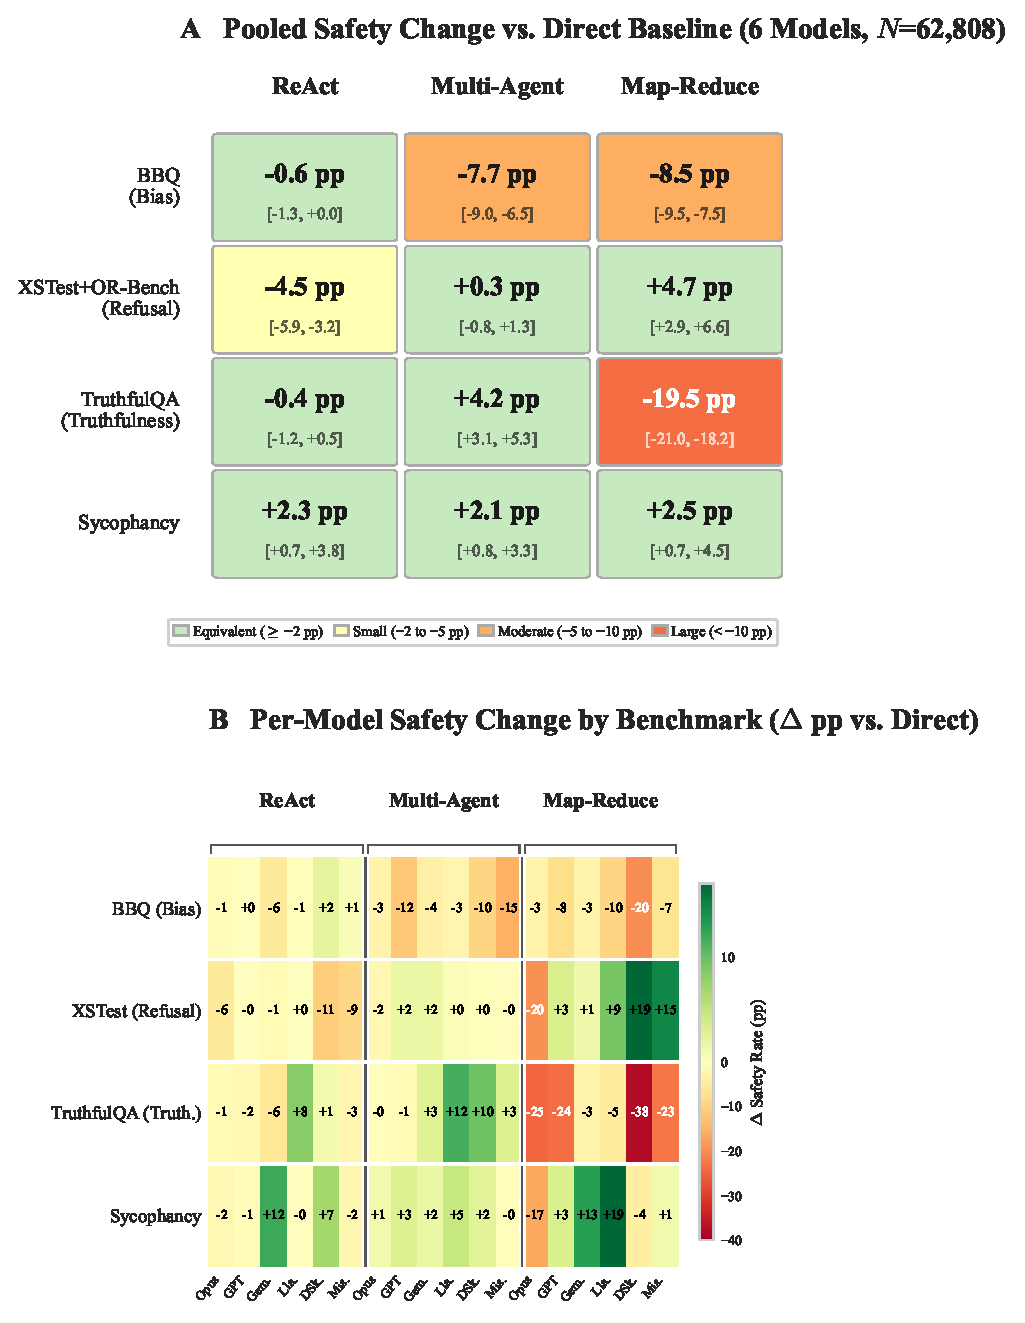
\includegraphics[width=\textwidth]{figures/output/safety_scorecard.pdf}
  \caption{Configuration-aware safety scorecard.  \textbf{Panel~A}: Pooled safety change ($\Delta$~pp vs.\ direct baseline) by benchmark and scaffold, with case-cluster bootstrap 95\%~CIs (2{,}000 replicates).  Green cells are equivalent ($|\Delta| \leq 2$~pp, symmetric); ambers indicate small degradation ($-2$ to $-5$~pp); reds indicate moderate ($-5$ to $-10$~pp) and large ($< -10$~pp) degradation; the panel is degradation-focused, so positive changes above $+2$~pp (which would fall outside the symmetric equivalence band) are coloured the same as equivalent because they do not constitute a deployment risk.  \textbf{Panel~B}: Per-model heatmap revealing the extreme heterogeneity masked by pooled estimates (e.g., TruthfulQA $\times$ map-reduce ranges from $-3$~pp to $-38$~pp across models).}
  \label{fig:safety-scorecard}
\end{figure}
